\documentclass{turabian-researchpaper}

\usepackage[utf8]{inputenc}
\usepackage{csquotes, ellipsis}
\usepackage{graphicx}
\usepackage{wrapfig}
\usepackage[pass, letterpaper]{geometry}
\usepackage{biblatex-chicago}
\addbibresource{works-cited.bib}

\title{Deviance Through the Divine}
\subtitle{An Analysis of Saint Hildegards Peculiar Rise to Power and Her Profound Illustrations}
\author{Ryan Heffelman}
\course{ARH-3760}
\date{October 26, 2023}

\begin{document}
\maketitle
\section{Introduction}
What does it take to be a successful historical female artist? In case of Saint Hildegard of Bingen, Divine Intervention.
In a truly one of a kind manner, Saint Hildegard literally transcended the gender constraints imposed upon her by a patriarchal
society, and she managed to do it in the most unlikely time and place imaginable; amongst devout religious people in the 1100s.
Saint Hildegard was not just a significant female artist, but a significant \emph{person}. In fact she's not even primarily known
for being an artist, more of a Saint, philosopher, visionary, theologian, etc. However this paper will focus on her illustrations.

\section{A Problem With the Interpretation of Saint Hildegard as an Artist}
In order to explain this problem I'd like to introduce a quote from Saint Hildegard's\autocite{scivias} Book I in reference to
a paragraph claiming God detests incest despite it being prevalent in the Old Testament:
"I am explaining this by this person [Hildegard], to whom this human operation is unknown; she is receiving this 
explanation not from human knowledge, but from God" \autocite[82]{scivias}. This is to say that her works are created by God through her as a proxy. 
God is expressing himself through her as a medium. If that's the case, then wouldn't that make her no more of an artist than 
Picasso's paintbrush is one?
Can \emph{she} really be seen as the artist of her works if it is God acting through her? Is this what allows her 
to remain in operation in a time and place so intolerant of female artists? One must tolerate her actions because her actions
are divine actions, to speak against her would be blasphemy. As far as I can see there are 2 ways around this problem, the
first of which being the Atheist way; the Catholic God is not real therefore God cannot be acting through her and her actions
are no ones but her own. The second way being the idea that while her illustrations are based on visions she experienced 
from God, she still went through the creative process of artistically representing what she's perceived, therefore
she is just as much an artist as any impressionist painter.

%\begin{figure}[h!]
    %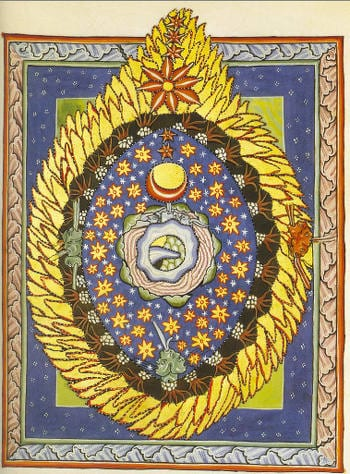
\includegraphics[width=0.4\linewidth]{C:/Users/ryanh/OneDrive/Documents/GitHub/ARH-3760/universe.jpeg}
    %\caption{``The Universe'' \emph{Scivias}.}\label{Figure A}
%\end{figure}
%\begin{figure}[h!]
    %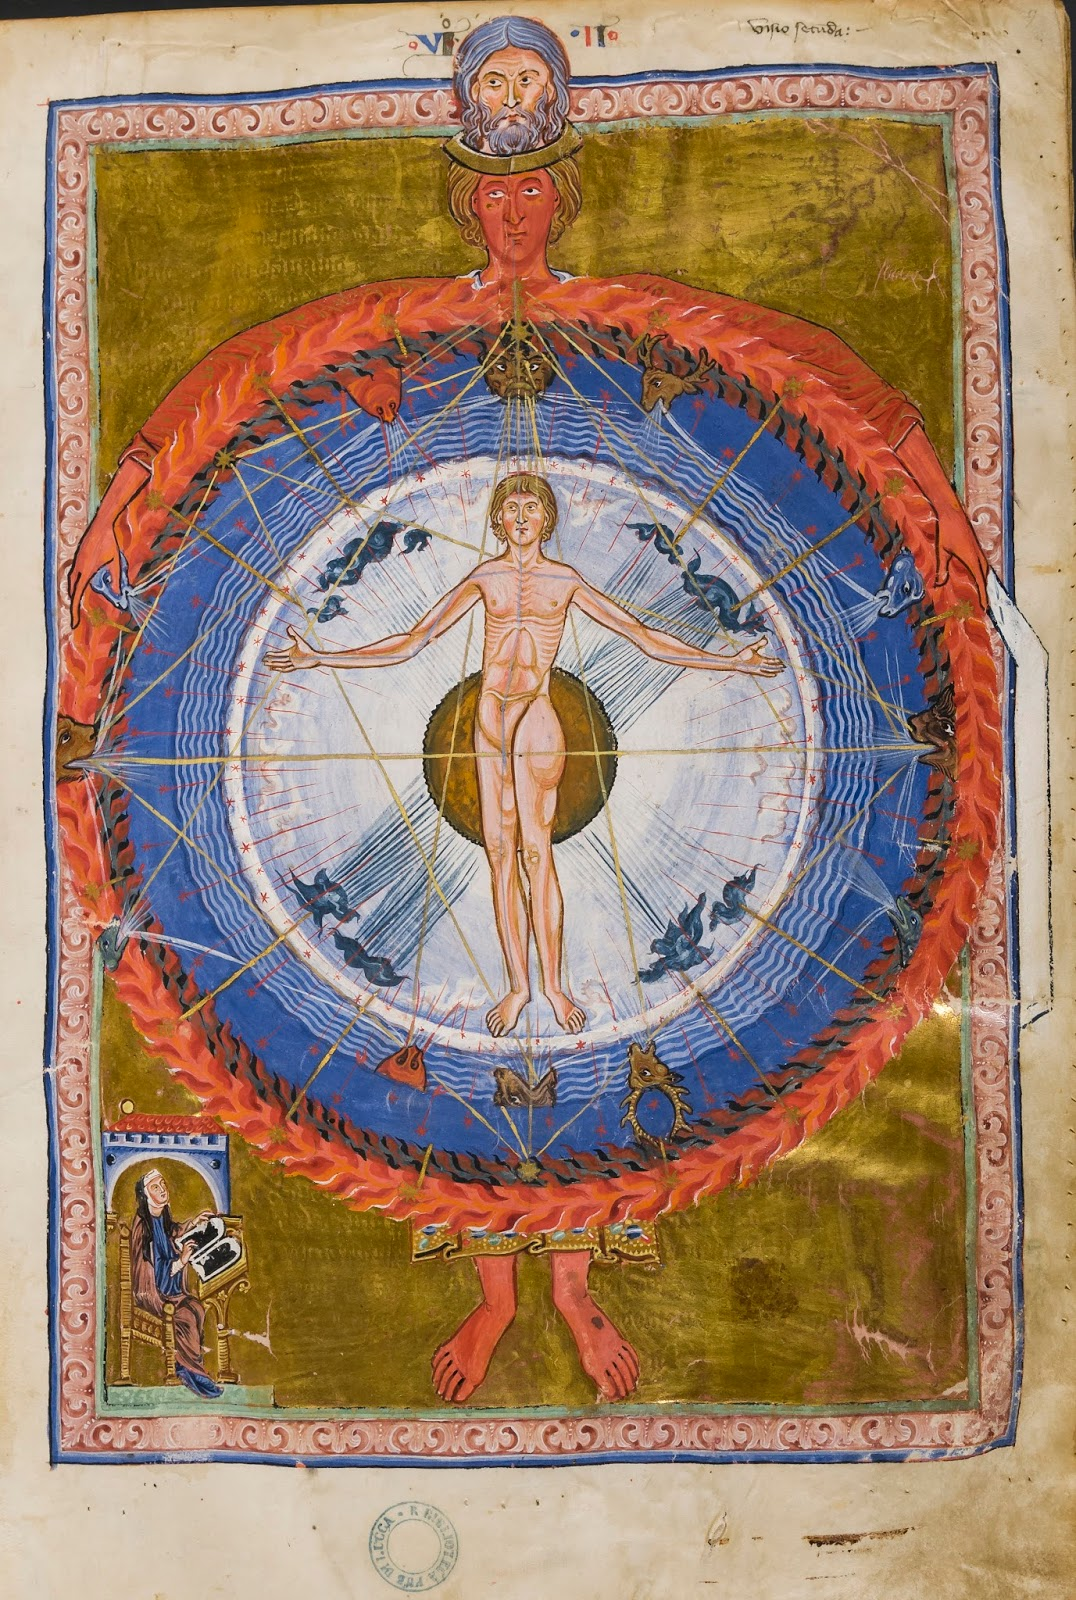
\includegraphics[width=0.4\linewidth]{C:/Users/ryanh/OneDrive/Documents/GitHub/ARH-3760/liber.jpg}
    %\caption{``The Universe'' \emph{Liber Divinorum Operum}.}\label{Figure A}
%\end{figure}

\section{Saint Hildegard's Astronomical legacy}
\begin{wrapfigure}{r}{0.4\textwidth}
    \centering
    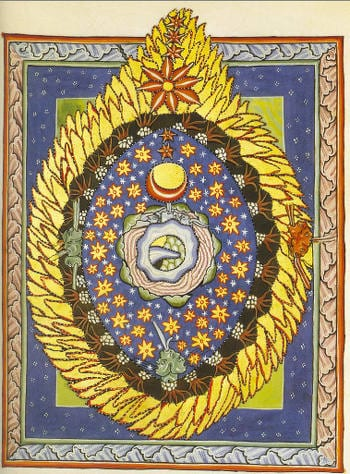
\includegraphics[width=\linewidth]{C:/Users/ryanh/OneDrive/Documents/GitHub/ARH-3760/universe.jpeg}
    \caption{``The Universe''}\label{Figure A}
\end{wrapfigure}

In midieval times, astronomy assumed a position of marked prominence. Saint Hildegard was a notable figure in many fields of 
medieval study, one of which being astronomy. In fact she's the only documented female astronomer
from the vast time period of the middle ages, this illustration of a model of the universe by a woman is one of a kind. (Figure 1)
When looking at any of her illustrations it is important to keep in mind that
they are designed to be interpreted through pictorial analogy as opposed to literal representation of described phenomena,
and her reasoning is almost exclusively \emph{a priori}.
This illustration is a demonstration that "The visible and temporal is a manifestation of the invisible and eternal" (Page 94),
an idea that resonates with the distinction between the Kantian phenomenal and the noumenal; the phenomenal domain implies
the existence of but 
says nothing about the noumenal domain. (Figure 1) The illustration represents a \emph{universal} union of the domains
with both being show


%\footnote{Some peripheral thoughts that belong in a note.}
\printbibliography
\end{document}
